\documentclass[11pt]{article}
\usepackage[margin=0.7in]{geometry}
\usepackage{multirow}
\usepackage {graphicx}
\usepackage[utf8x]{inputenc} % указать кодировку русского текста
\usepackage[russian]{babel} % указать, что язык текста - русский
\usepackage{fancyhdr}
\pagestyle{fancy}
\usepackage{graphicx}
\graphicspath{{pictures/}}
\DeclareGraphicsExtensions{.pdf,.png,.jpg}
\begin{document}
\begin{titlepage}
\begin{center}
\large\textbf{Московский Физико-Технический Институт}\\
\large\textbf{(государственный университет)}
\vfill
\huge\textbf{ Работа 3.5.1}\\
\huge\textbf{Изучение плазмы газового разряда в неоне}\\
\vfill
\large Факультет электроники, фотоники и молекулярной физики\\
\end{center}
\end{titlepage}
\fancyhead[L] {Работа 3.5.1}
\noindent \textbf{Цель работы:} \\
\indent изучение вольт-амперной характеристики тлеющего разряда; изучение свойств плазмы методом зондовых характеристик.\\
\noindent \textbf{В работе используются:} \\
\indent стеклянная газоразрядная трубка, наполненная неоном; высоковольтный источник питания; источник питания постоянного тока; делитель напряжения; потенциометр; амперметры; вольтметры; переключатели.
\section*{Описание работы}\
\emph{Газовый разряд} - любой процесс возникновения ионизации газа под действием приложенного электрического поля.\\
Введём понятие \emph{дифференциального сопротивления} как производную от напряжения по току:
$$R_{diff} = \frac{dU}{dI}$$
Характерной особенностью вольт-амперной характеристики газового разряда, не свойственной обычным проводникам, являются участки с отрицательным дифференциальным сопротивлением, $R_{diff} < 0$. Такие участки называются неустойчивыми: незначительное уменьшение подаваемого на элемент напряжения приводит к росту тока - и поскольку для поддержания возросшего тока требуется ещё меньшее напряжение, это провоцирует неограниченный рост тока.\\
\section*{Экспериментальная установка}
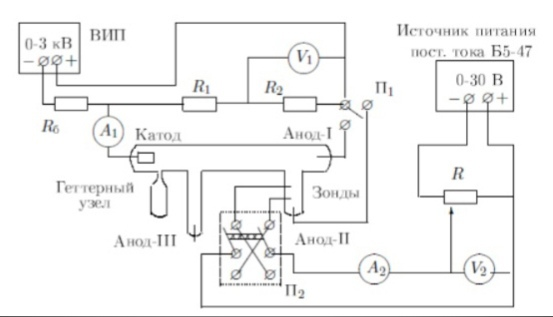
\includegraphics[width = 16cm]{3511}\\
Параметры зонда:\\
$d = 0,2mm$\\
$l = 5,2mm$\\
\section*{Ход работы}\
1.С помощью вольтметра V1 и амперметра A1 измерим вольт-амперную характеристику разряда $I_{raz}(U_{raz})$. Проводим две серии измерений: при нарастании и при убывании тока.\\
Для начала определим напряжение зажигания разряда: $U_{z}= 215 \pm 3$ B - такая погрешность взята из соображений реакции челолвеческого глаза на зажигание.\\

\textbf{Таблицы значений:}\\
\ \\
На убывание:\\
\begin{tabular}{|l|l|}
\hline
I, mA, $\sigma_I=0,02$ mA & U, В, $\sigma_U$ = 0,1 В\\
\hline
4,76 & 15,8
\\
\hline
4,32 & 16,1
\\
\hline
3,80 & 16,9
\\
\hline
3,20 & 18,7
\\
\hline
2,8 & 18,6
\\
\hline
2,36 & 19,9
\\
\hline
1,96 & 22,4
\\
\hline 
1,52 & 29,8
\\
\hline
1,20 & 33,4
\\
\hline
0,96 & 34,0
\\
\hline
0,64 & 34,5
\\
\hline
0,24 & 35,6
\\
\hline
0 & 51,2
\\
\hline
\end{tabular}
\ \\
На возрастание:\\
\begin{tabular}{|l|l|}
\hline
I, mA, $\sigma_I=0,02$ mA & U, В, $\sigma_U$ = 0,1 В\\
\hline
2,04 & 21,8
\\
\hline
2,36 & 20,2
\\
\hline
2,52 & 19,0
\\
\hline
2,80 & 18,8
\\
\hline
3,0 & 19,1
\\
\hline
3,24 & 18,7
\\
\hline
3,52 & 17,8
\\
\hline 
3,84 & 16,9
\\
\hline
4,0 & 16,6
\\
\hline
4,20 & 16,3
\\
\hline
4,4 & 16,1
\\
\hline
4,64 & 15,9
\\
\hline

\end{tabular}
\ \\
\textbf{Построение графиков:}\\
\ \\
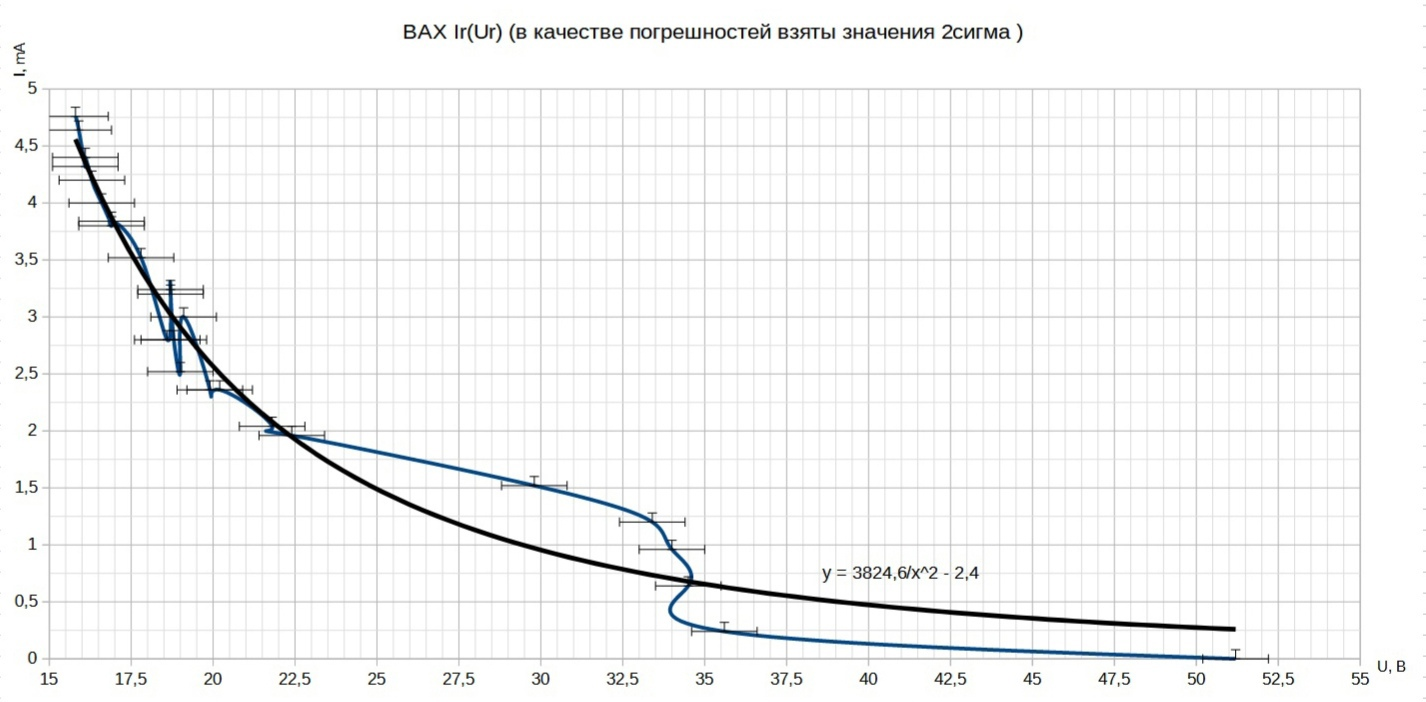
\includegraphics[width = 19cm]{vah}\\
\em Измерение погрешностей \em: \\
Исходный график напоминает функциональную зависимость $\sim k/x^(2) + b$\\. Проверим это предположение, посчитав МНК именно для неё и построив аппроксимирующую кривую:\\
$$ y = \frac{k}{x^2} + b $$
$$ b = <y> - k<\frac{1}{x^2}> $$
$$ k = \frac{<y\frac{1}{x^2}> - <y><\frac{1}{x^2}>}{<\frac{1}{x^4}> - (<\frac{1}{x^2}>)^2} $$
$$ \sigma_{k} = \sqrt{\frac{1}{n-1}(\frac{<y^2> - (<y>)^2}{<\frac{1}{x^4}> - (<\frac{1}{x^2}>)^2} - k^2} $$
$$ \sigma_{b} = \sigma_{k}\sqrt{<\frac{1}{x^4}> - (<\frac{1}{x^2}>)^2} $$
\\
$$  k = \frac{0,00853 - 0,007}{0,0000076 - 0,0000072} \approx 3824,6  $$
$$ b = 2,73 - 3825\times 0,00135 \approx -2,43 \approx -2,4 $$
$$ \sigma_{k} = \sqrt{\frac{1}{25}(\frac{9,339 - 7,45}{0,0000076 - 0,0000072} - 3824,6^2} \approx 87 $$
$$ \sigma_{b} = 87\sqrt{0,0000076 - 0,0000072} \approx 0,06$$
Итоговая аппроксимирующая кривая:\\
\fbox{$y = 3824,6\frac{1}{x^2} - 2,4$}\\
\\
Перестроим ВАХ в координатах $U(I)$, чтобы можно было проще найти максимальное дифференциальное сопротивление разряда.
По наклону кривой определим максимальное дифференциальное сопротивление разряда:\\
$ R_{diff} = \frac{dU}{dI}$
Касательная к кривой с максимальным наклоном имеет вид: $ y = -65x + 51,2$. Поэтому $R_{diff} = 6,5 \times 10^4$ Ом\\
Рассчитаем погрешность данной величины:\\
$$(\sigma_{R}/R)^2 = (\sigma_{U}/U)^2 + (\sigma_{I}/I)^2$$
$$ \sigma_{R}/R \approx 0,06 $$
$$ \sigma_{R} \approx 0,4 \times 10^4 Om $$
Поэтому итоговое дифференциальное сопротивление \fbox{$R_{diff} = (6,5 \pm 0,4) \times 10^4 Om $}\\

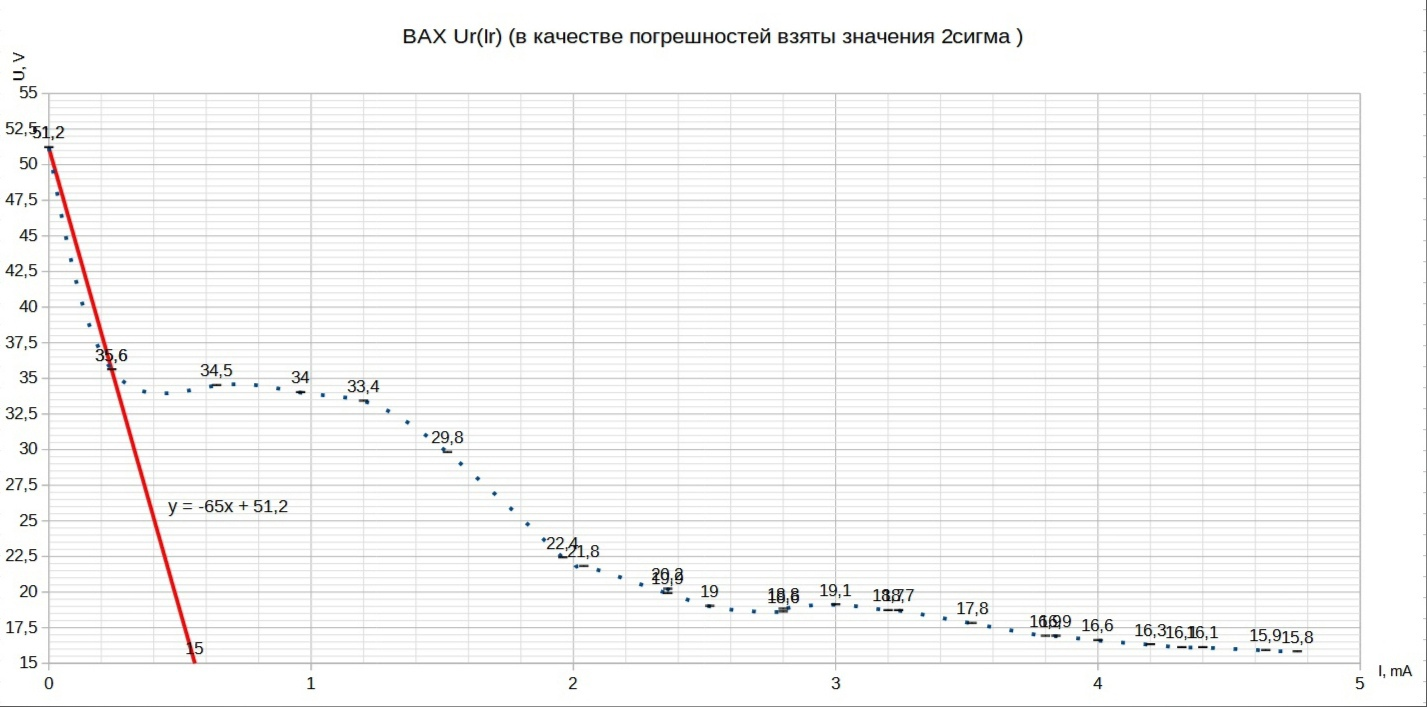
\includegraphics[width = 19cm]{vahk}\\
\\
2. Снимем ВАХ двойного зонда $I_z(U_z)$ при различных фиксированных токах разряда $I_r$ в диапазоне -25 $\div$ 25 В:\\
а) $I_r = 5 mA$\\
\begin{tabular}{|l|l|l|l|}
\hline
I, mkA, $\sigma_I = 0,1$ mkA & U, B, $\sigma_U = 0,1$ (положит.пол) & I, mkA, $\sigma_I = 0,1$ mkA & U, B, $\sigma_U = 0,1$ (отриц.пол)\\
\hline
110,9 & 24,9 &118,4 &-25
\\
\hline
108,4 & 21,8 & 117,2 & -23,7
\\
\hline
105,3 & 18,5 & 116 & -22,4
\\
\hline
101,7 & 15,7 & 114,4 & -20,7
\\
\hline
96,3 & 12,9 & 112,4 & -18,8
\\
\hline
89,2 & 10,5 & 110,1 & -17,1
\\
\hline
82,3 & 8,8 & 107,2 & -15,5
\\
\hline
75,7 & 7,5 & 105,1 & -14,4
\\
\hline
66,7 & 6,0 & 101,4 & -12,9
\\
\hline
61,9 & 5,3 & 95,8 & -11,2
\\
\hline
53,4 & 4,2 & 90,7 & -10,1
\\
\hline
47,8 & 3,6 & 84,0 & -8,7
\\
\hline
43,5 & 2,9 & 76,5 & -7,3
\\
\hline
31,9 & 1,65 & 67,5 & -6,0
\\
\hline
23,9 & 0,95 & 58,2 & -4,8
\\
\hline
19,1 & 0,3 & 49,1 & -3,8
\\
\hline
107,6 & 19,8 & 40 & -2,6
\\
\hline
108,2 & 20,4 & 30,3 & -1,5
\\
\hline
110,7 & 23,2 & 22,8 & -0,9
\\
\hline
107,7 & 16,6 & 14,1 & -0,1
\\
\hline
99,2 & 13,8 & &
\\
\hline

\end{tabular}
\\
\\
б) $I_r = 3 mA$\\
\begin{tabular}{|l|l|l|l|}
\hline
I, mkA, $\sigma_I = 0,1$ mkA & U, B, $\sigma_U = 0,1$ (положит.пол) & I, mkA, $\sigma_I = 0,1$ mkA & U, B, $\sigma_U = 0,1$ (отриц.пол)\\
\hline
59,8& 25 &-62,1 &-25
\\
\hline
59,2 & 23,8 & -61,3 & -23,8
\\
\hline
57,6 & 21,1 & -60,2& -21,8
\\
\hline
56,6 & 19,3 & -58,8 & -19,4
\\
\hline
55,2 & 16,9 & -57,7 & -17,6
\\
\hline
53,7 & 14,7 & -55,9 & -15,0
\\
\hline
52,4 & 13,3& -54,6& -13,6
\\
\hline
51,1 & 11,9& -52,5 & -12,0
\\
\hline
47,5 & 10& -49& -10,1
\\
\hline
42,9 & 8,2 & -42,4 & -7,8
\\
\hline
40,0 & 7,2 & -38,2& -6,6
\\
\hline
35,9 & 6,1 & -30,2& -4,9
\\
\hline
29,1 & 4,5 & -25,1& -3,8
\\
\hline
22,1 & 3,2 & -18,4& -2,6
\\
\hline
13,7 & 1,8 & -12,2& -1,6
\\
\hline
8,3 & 0,9& -7,2& -0,8
\\
\hline
3,6 & 0,1 & -2,7& -0,1
\\
\hline
\end{tabular}
\\
\\

в) $I_r = 1,5 mA$\\
\begin{tabular}{|l|l|l|l|}
\hline
I, mkA, $\sigma_I = 0,1$ mkA & U, B, $\sigma_U = 0,1$ (положит.пол) & I, mkA, $\sigma_I = 0,1$ mkA & U, B, $\sigma_U = 0,1$ (отриц.пол)\\
\hline
28,0& 25 &-29,3 &-25
\\
\hline
27,6 & 23,7 & -28,6 & -23
\\
\hline
26,9 & 21,6 & -28,1& -21,4
\\
\hline
26,5 & 20,4 & -27,8 & -20,3
\\
\hline
26,3 & 19,3 & -27,1 & -18,4
\\
\hline
25,8 & 17,8 & -26,6 & -17
\\
\hline
25,3 & 16,2& -26& -15,4
\\
\hline
24,9 & 15,1& -25,7 & -14,5
\\
\hline
24,3 & 13,7& -25,1& -13,3
\\
\hline
23,0 & 11,4 & -24,2 & -12
\\
\hline
21,4 & 9,6 & -23,0& -10,4
\\
\hline
20,0 & 8,3 & -21& -8,8
\\
\hline
18,1 & 7,0 & -19,2& -7,6
\\
\hline
16,1 & 5,9 & -16& -5,8
\\
\hline
14,2 & 4,9 & -13,5& -4,7
\\
\hline
11,5 & 3,7& -10,6& -3,6
\\
\hline
8,6 & 2,6 & -8,3& -2,8
\\
\hline
4,8 & 1,5 & -5,0& -1,6
\\
\hline
2,1 & 0,7 & -3,0& -0,9
\\
\hline
0,4 & 0,1& -1,7& -0,5
\\
\hline
& & -0,2 & -0,1
\\
\hline
\end{tabular}
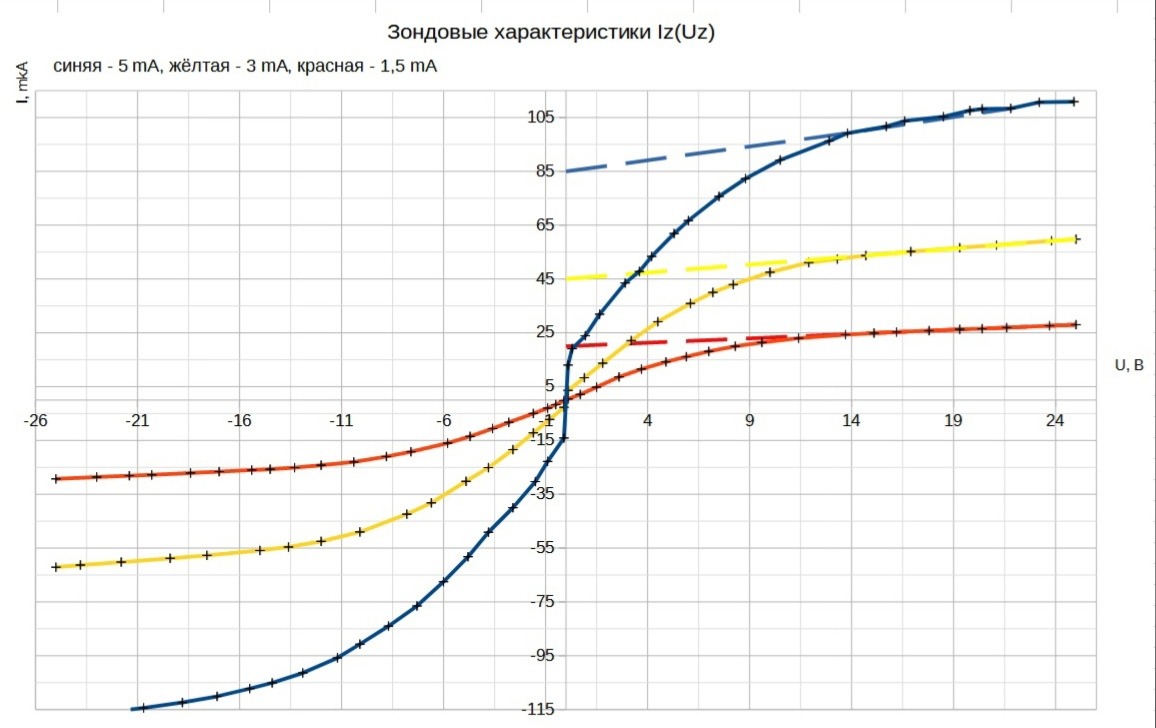
\includegraphics[width = 19.5cm]{vahz}\\
Далее по каждой зондовой характеристике определяем:\\
а) ионный ток насыщения $I_{in}$ по пересечению асимптот к графику, проведенных при $U_{z} \rightarrow \pm U_{zmax}$, с осью ординат\\
б) наклон характеристики $dI/dU(U = 0)$ в начале координат\\
Результаты занесём в таблицу для каждой из характеристик:\\
\\
\begin{tabular}{|l|l|l|l|}
\hline
 & 5 mA & 3 mA & 1,5 mA\\
\hline
$I_{in}, \pm 0,02 mA$ mkA& 85 &45 &20
\\
\hline
$dI/dU(U = 0), 10^{-6} A/V$ & 25,1 $\pm$ 4,2 & 9,2 $\pm$ 1,7 & 3,3 $\pm$ 0,6
\\
\hline
\end{tabular}
\\
\\
По результатам предыдущего пункта найдем температуру электронов $T_{e}$ в Кельвинах по формуле:\\
$ kT_{e} = \frac{1}{2}\frac{eI_{in}}{dI/dU(U = 0)}$\\
\begin{tabular}{|l|l|l|l|}
\hline
 & 5 mA & 3 mA & 1,5 mA\\
\hline
$kT_{e}, $ эВ & 1,7$\pm 0,3$ & 2,4 $\pm 0,5$ & 3,0 $\pm 0,6$
\\
\hline
$T_{e}, 10^3 K $ (1 эВ $\simeq 11800$ К) & 20 $\pm 2$ & 28,3 $ \pm 4,1$ & 35,4 $\pm 5,7$
\\
\hline
\end{tabular}
\\
\\
Полагая концентрацию электронов $n_e$ равную концентрации ионов $n_i$, определим её по формуле Бома:\\
$I_{in} = 0,4n_{e}eS\sqrt{\frac{2kT_{e}}{m_{i}}}$\\
Сделав расчёт размерностей, понимаем, что удобнее всего будет считать в $10^{15} m^{-3} $\\
\begin{tabular}{|l|l|l|l|}
\hline
 & 5 mA & 3 mA & 1,5 mA\\
\hline
$n_{e}, 10^{15} m^{-3}$ & 133,3 $\pm 60,1 $& 70,6 $\pm 30,2$ & 31,4 $\pm 14,7$
\\
\hline
\end{tabular}
\\
\\
Далее рассчитаем плазменую частоту колебаний электронов по формуле:\\
$ \omega_{p} = \sqrt{\frac{4\pi n_{e}e^2}{m_{e}}} \approx 5,6 \times 10^4 \sqrt{n_{e}} $ рад/сек\\
\\
\begin{tabular}{|l|l|l|l|}
\hline
 & 5 mA & 3 mA & 1,5 mA\\
\hline
$\omega_{p}, 10^{13} rad/sec$ & 64,6 $\pm 4,3$ & 47,1 $\pm 5,2$ & 31,4 $\pm 4,9$
\\
\hline
\end{tabular}
\\
\\
Рассчитаем электронную поляризационную длину $r_{de}$ по формуле:\\
$ r_{de} = \sqrt{\frac{kT_{e}}{4\pi n_{e}e^2}}$ м\\
\begin{tabular}{|l|l|l|l|}
\hline
 & 5 mA & 3 mA & 1,5 mA\\
\hline
$ r_{de} $, $10^{-2}$ м & 6,3 $ \pm 0,7$ & 17 $\pm 2,3$ & 47 $\pm 5,1$
\\
\hline
\end{tabular}
\\
\\
Рассчитаем дебаевский радиус экранирования $r_{d}$:\\
$ r_{de} = \sqrt{\frac{kT_{i}}{4\pi n_{e}e^2}}$\\
\begin{tabular}{|l|l|l|l|}
\hline
 & 5 mA & 3 mA & 1,5 mA\\
\hline
$ r_{d} $, $10^{-4}$ м & 9,7 $\pm 1,2$ & 18 $\pm 2,5$ & 41 $\pm 5,0$
\\
\hline
\end{tabular}
\\
\\
Оценим среднее число ионов в дебаевской сфере:\\
$ N_{d} = \frac{4}{3}\pi (r_{d})^3n_{i}$\\
\\
\begin{tabular}{|l|l|l|l|}
\hline
 & 5 mA & 3 mA & 1,5 mA\\
\hline
$ N_{d} $, $10^{5}$  & 5,1 & 17,2 & 90,6
\\
\hline
\end{tabular}
\\
\\
Так как число Дебая получилось >>1, то плазму можно считать идеальной.\\
Оценим степень ионизации плазмы:\\
\\
\begin{tabular}{|l|l|l|l|}
\hline
 & 5 mA & 3 mA & 1,5 mA\\
\hline
$ \alpha$,$10^{-7}$ & 20,8 & 11 & 4,9
\\
\hline
\end{tabular}
\\
\\
(погрешности везде в этом пункте считались по формулам погрешности отношения и произведения)\\
Построим графики зависимостей электронной температуры и концентрации электронов от тока разряда: $T_{e}(I_{p}), n_{e}(I_{p})$\\
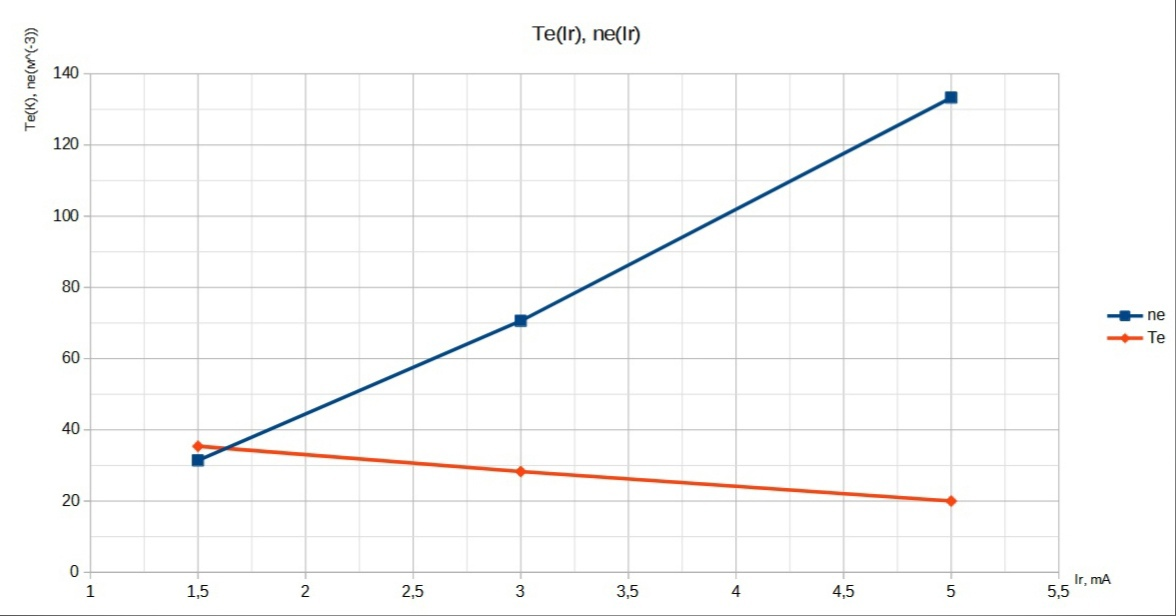
\includegraphics[width = 19.5cm]{zav}\\
\newpage
\subsubsection*{Вывод:}
Полученные результаты по порядку, (либо отличаются на порядок) совпадают с табличными данными из интернета. Разница могла возникнуть из-за того, что вблизи нуля зондовые характеристики (ВАХ) снимались не очень тщательно и точек было мало.\\


\end{document}